\chapter{L’haptique au service de la médecine / prothèses DIY }
\section{Introduction}
je vais refaire l'intro en fonction de son qu'on a dit durant l'appel 

\textit{Prostheses}

The use of haptics for therapeutic purposesA prosthesis is an artificial device designed to replace a limb, organ, or joint. The term "prosthesis" comes from the Greek word "prosthesis," meaning "the act of adding." The field of prosthetics is considered interdisciplinary, situated at the intersection of engineering, medicine, and biology. It encompasses the design, development, and manufacture of artificial devices intended to replace or enhance the functions of human limbs or other body parts. Modern prostheses go beyond merely replacing the mechanical process of a lost limb. They also contribute to patients' physical and mental rehabilitation by helping them resume their daily and professional activities [1].

Numerous prostheses exist today, varying in their design, components, and functionality. There are purely aesthetic prostheses designed to visually replace a missing part of the body [2]. Mechanical [3], myoelectric [4], or hydraulic [5] prostheses use different means, such as electrical signals or fluids (liquids or gases), to control the prosthesis and perform precise movements similar to human motion.

Advanced projects focus on neuroprosthetics. Cutting-edge research concentrates on creating neural interfaces that enable direct communication between the prosthesis and the user's brain [6]. The prosthesis allows for more intuitive control of the prosthetic limb's movements, bridging the gap between the user's intentions and the limb's actions.

\textit{BioMaterials and BioPatches}

Innovation is crucial in enhancing patient care and seeking more effective treatment solutions in the medical field. Biomaterials and biopatches have emerged as essential areas of research and innovation at the intersection of engineering, medicine, and materials science.

Biomaterials, a class of materials designed to interact harmoniously with biological systems, have catalyzed a revolution in regenerative medicine, surgery, and personalized medicine. Their versatility enables the creation of more advanced prosthetics and implants [7], tissue regeneration [8], and controlled drug release [9]. They have transformed how we approach the design of medical devices and surgical interventions, providing new opportunities to enhance human health.

Simultaneously, biopatches [10], a specific application of biomaterials, have proven to be valuable tools for tissue regeneration, targeted drug delivery, and real-time monitoring of physiological parameters [11]. Known as skin patches, they have evolved from simple adhesive bandages to sophisticated and multifunctional devices. They combine sophisticated biomaterial properties with cutting-edge technologies, opening new perspectives in fields ranging from regenerative medicine to wearable medical monitoring.

The interest in biopatches and biomaterials stems from the desire to improve the quality of life for patients by offering more comfortable and less invasive alternatives to traditional treatments. These areas hold revolutionary potential to enhance individuals' quality of life, transform healthcare, and pave the way for extraordinary medical advances.

This project aims to make the design of bioplastics, biopatches, prostheses, and prosthetic enhancements more accessible to the general public. It focuses on rapid and cost-effective prototyping while providing essential knowledge in the design and manufacturing methods of DIY biopatches and prostheses. It serves as an initial step for anyone interested in engaging in these fields, offering straightforward and affordable solutions to enhance the daily lives of amputees.

\section{Related Work}

\textit{Prostheses}

The field of prosthetics has witnessed incredible advancements driven by cutting-edge engineering technologies. These developments encompass design, materials, sensor integration, neurology, and accessibility.

Some projects are moving towards personalization. Recent trends emphasize the creation of tailored solutions. With 3D printing and scanning technologies, prosthetics can be custom-made to match the user's unique anatomy, enhancing comfort and functionality. Projects like that of David C. Ackland and his team [1] develop custom 3D-printed prosthetic joints based on scans. Similarly, Naomi C. Paxton and her team [2] craft customized prosthetics after an in-depth patient anatomy study.

In addition to customization and 3D printing, there is a growing focus on patient autonomy. An increasing number of projects offer prosthetics for personal assembly (Do It Yourself, DIY), enabling individuals to design their prostheses. It's exemplified by initiatives such as My Human Kit and Bionicohand [3], which provide detailed tutorials with accessible files for creating personalized forearm prosthetics using 3D printing, a technology within reach of most. Movements like E-nable [4] actively promote this concept and encourage self-reliance.

Others are dedicated to incorporating lightweight, durable, and biocompatible materials, contributing to developing more comfortable and functional prosthetics. In 1974, researcher Sauer and his team [5] explored using porous polyethylene, which can adapt to tissue growth when manufactured in this form. Subsequently, other projects have continued to explore material choices [6][7]. M.-S. Scholz and his team [8] have focused on using composites with an excellent strength-to-weight ratio and outstanding biocompatibility. All these projects aim to mimic the mechanical properties of natural limbs, promoting a more natural and efficient approach.

Sensor integration represents a significant part of prosthetic innovation. Sundaram and his team [9] developed a glove demonstrating that sensors uniformly distributed on the hand can identify individual objects, estimate their weight, and explore the typical tactile patterns that emerge when grasping objects. Prosthetic limbs equipped with various sensors enable users to perceive their environment better. These sensors provide real-time information, such as pressure, temperature, and movement, enhancing the user's awareness and control over the prosthetic limb [10]. Projects like those led by Ting Zhang and his team [11], or Low. C and his colleagues [12] showcase the integration of tactile sensors, allowing users to manipulate delicate objects more effectively and regain a sense of touch lost due to amputation.

\textit{BioMaterials and BioPatches}

With the emergence of bio-materials, bio-patches technology has arisen as a revolutionary field in medical devices, potentially transforming the way medical treatments are administered and monitored.

In terms of materials, some projects focus on composite bio-materials. The project led by Román A. Pérez and al. [13] creates bio-materials that stimulate/trigger targeted cellular responses critical in tissue regeneration processes. Bio-materials combine different materials to harness their specific properties and are commonly used. For instance, polymer-ceramic composites find applications in dental implants [14].

Integrating electronics into bio-materials and bio-patches is a significant part of the innovation in this field. Eldy Vasquez and al. project [15] explores using mycelium with standard digital fabrication techniques to replace plastics in electronics. Bio-materials are now being designed to incorporate electronics, opening up possibilities in intelligent medical devices [16]. Polymeric bio-materials serve as integral components, including thin-film electronics, in vitro cell culture models, and implantable medical devices [17].

The project by Logesh S and al. [18] employs a double-layered plant-based bio-polymeric patch (bio-patch) with wound healing efficacy and skin-mimicking functions for cutaneous tissue regeneration applications. Enhancing bio-compatibility is a crucial aspect of bio-patch innovation. Researchers are striving to improve the bio-compatibility of bio-materials to reduce immune reactions and minimize the risk of rejection.

Many of these projects are environmentally and sustainability-conscious. There is a growing interest in developing eco-friendly and sustainable bio-materials, focusing on waste reduction and using renewable resources.

Despite the wide range of applications and processes, these techniques still need to be simplified for inexperienced users. They either require the use of expensive equipment, the modification and design of machinery, or extensive knowledge in other fields such as mechanics, design, medicine, or even biochemistry. On the other hand, the project presented in this chapter does not demand advanced knowledge. It relies on simple and cost-effective methods and components, enabling the creation of a self-contained prototype.

\section{Prosthetics DIY}

\subsection{Objectives}

The objective of this 3D design is to provide support for the various haptic components used and to complement a forearm prosthesis. While it is possible to modify an existing prosthesis, this requires 3D design skills on the part of the user and may appear complex due to the wide variety of available prostheses. To accompany the DIY haptic kit, we offer a simple device. It is added to a prosthesis and positioned at different locations on the arm to accommodate various types of amputations. Its design aims to maximize accessibility and facilitate printing or modifications as needed. It allows for integrating multiple components while reducing the bulk they bring.

\subsection{Materials Used}
The use of 3D printing has become increasingly common in the field of prosthetics, primarily due to its flexibility, customization, and production speed. Here is a list of materials commonly used in 3D printing that we have explored for the creation of an additional device to the kit:

PLA, or Polylactic Acid, is one of the most popular materials in 3D printing, especially for beginners. It is known for its ease of printing. Due to its biological origin, PLA is usually considered bio-compatible, making it suitable for applications such as creating prosthetics or temporary medical implants. Moreover, it’s one of the least expensive materials for 3D printing, making it a cost-effective choice for beginners and experimental projects. However, it has heat resistance and mechanical strength limitations, which can restrict its use in high-performance applications.

ABS, or Acrylonitrile Butadiene Styrene, is commonly used in 3D printing. His toughness and durability make it a popular choice for various applications. It is known for its mechanical strength and shock resistance, meaning it can withstand high loads and stresses. Furthermore, it can be easily sanded and polished to achieve a smooth and aesthetic finish. However, it can emit toxic fumes and is not biodegradable. ABS is widely used in industrial part production, mechanical components, and functional prototypes. 

Polypropylene (PP) is a thermoplastic widely used in 3D printing due to its distinctive characteristics, lightweight nature, and durability. Polypropylene is one of the lightest plastics in 3D printing, making it suitable for low-density applications. Polypropylene absorbs very little moisture and exhibits high shock resistance, making it ideal for parts subjected to mechanical stress. However, printing can be challenging and may require specific settings and a compatible printer.

TPU, or Thermoplastic Polyurethane, is a material appreciated in 3D printing for its flexibility, impact resistance, and versatility. Additionally, it’s often considered bio-compatible, making it a choice for medical applications and skin contact parts. It effectively resists abrasion, making it suitable for parts prone to wear. However, TPU can be challenging to print due to its elasticity and is generally more expensive than more familiar materials like PLA or ABS.

Nylon is a popular 3D printing material known for its strength and durability. While it is less flexible than TPU, nylon has some flexibility, making it suitable for applications requiring slight deformation. It can be used in various applications, from prototypes to final parts. However, nylon tends to absorb moisture from the air, requiring pre-print drying to avoid issues. It is generally more expensive than common materials like PLA or ABS.

The choice of material will depend on the specific needs of each prosthesis, including the intended function, durability, flexibility, and bio-compatibility. Many tests and prototyping have been conducted to determine the most suitable material.

\subsection{Modeling}

The kit’s various components, projects, and prototypes intended for material testing were created using different modeling software. Among them, we find SolidWorks, a modeling software well-known to the general public, and nTopology, a widely used software in medicine for designing lattice structures and complex geometries.

Scans were performed on forearms, feet, and amputated limbs using the Ossür software to enable the printing of amputee sockets, braces, and orthopedic insoles and to conduct material tests.

Orthopedic insoles, sockets, and braces are created from scans and modeled in nTopology. In contrast, prostheses and elements of the DIY kit are designed using SolidWorks.

\subsection{Implementation}

Several prototypes were created, whether to evaluate materials or assess ease of printing and usage. In this regard, auxiliary projects were undertaken, including the design of splints, sockets, and orthopedic insoles tested on patients. Each project presented a unique challenge with specific requirements, enabling the evaluation of materials based on various criteria such as strength, flexibility, cost, and more.

\textit{Prototyping for the Kit}
\item Objectives

The first step in the kit involves modifying an accessible online prosthesis. This choice was made due to its simplicity as an initial trial for the KIT. The goal was to find a removable prosthesis that was accessible to all and easily adaptable.

\item Modeling and Implementation

The main modification concerns the platform holding the cables responsible for finger movement in the prosthesis. It was adapted to accommodate all necessary microcontrollers. The basic structure is retained, but a second level was added to attach a PCB with the components, which can be directly affixed to the platform. The primary aim of this prototype was to integrate these components to ensure ergonomic usability without hindering the user during kit and prosthesis use.

This first prototyping is simple but requires further use. It has been developed to test the various components better to understand the needs and constraints for a second proposal. PLA is a suitable material for this device. 

\textit{Kit Device}
\item Objectives

The second prototype is a device designed to complement a forearm prosthesis. It is simpler to reach a broader audience by providing a device that can be added to an existing prosthesis rather than attempting to modify a prosthesis used by a small number of individuals and potentially not meeting their specific needs. This concept underpins the design of the second device.

\item Modeling and Implementation

Its design is based on a device positioned on the arm, whether on the forearm or the upper part beyond the elbow. Similar to a bracelet, it wraps around the arm. The base diameter is adjustable in the design phase or directly based on the chosen material's flexibility. The top part is flat and hollow, accommodating the PCB with various controllers required for the kit. Holes are provided for routing cables connecting sensors to microcontrollers, and notches on the sides allow the device to be fastened to the arm using Velcro.

This device stands out for its design, modification, and use simplicity. Its geometry allows it to be printed with various materials, eliminating the risk of poor printing. Its purpose is not to replace or modify an existing prosthesis but to complement it, ensuring compatibility with a wide range of prosthesis types. For this device, ABS and nylon are recommended for their strength, while PP offers excellent flexibility and ease of movement.

\textit{Device for Various Sensors}
\item Objectives

In addition to the device for supporting controllers, another device was conceived to attach various types of sensors. It should be user-friendly and compatible with a wide range of prostheses. In addition to the platform designed to support controllers, another device intended to attach various types of sensors was envisioned. It should be accessible and adaptable to as many prostheses as possible.

\item Modeling and Implementation

The design of this device follows the same principle as the previous one. It is an open ring designed to slide onto the end of the prosthesis, allowing it to be positioned on the prosthetic finger. TPU is strongly recommended for its high flexibility. A flat base, bordered by right-angled edges, allows for the insertion of various sensors. For circular piezoelectric sensors, the bottom has a corresponding circular shape.

In addition to these various devices, using highly flexible electrical wires to connect different components is highly recommended. They offer the ability to track the user's movements without the risk of breaking, such as Adafruit Stainless Thin Conductive Yarn for sewing.


\section{Bio-Patches}
\subsection{Concept}
The goal of this chapter is simple: to provide a simple process for creating bio-patches. By exploring various materials and manufacturing techniques, this section offers a practical DIY guide for bio-patch fabrication. Each patch will consist of two distinct layers. The lower layer will directly contact the skin, while an upper layer will cover it. A haptic motor is inserted between these two layers to prevent direct contact with the skin. 

\subsection{Constraints}
The production of these bio-patches has presented several constraints:

Firstly, there are mechanical constraints. These patches must withstand various mechanical forces such as pressure, stretching, and torsion. They must not tear, remain adequately flexible, and be capable of stretching to follow the movements once applied to the individual's arm. Tear resistance is a mechanical property that measures a material's ability to resist the propagation of cracks. There is no single mathematical formula to calculate this resistance because it depends on various factors, including the sample's geometry, loading conditions, the material's properties, and more.

Next, there are constraints related to attaching the patch to the individual's arm. The part in contact with the skin must be adhesive enough to stay in place, while the outer layer must resist the friction caused by clothing. Friction is the force that opposes motion when one object's surface comes into contact with another. Its magnitude depends on the size of the contacting covers, textures, the forces involved, as well as the angle and position of the object (figure … ).

Finally, there are constraints related to manufacturing and accessibility. We seek a patch that is durable, easy to produce, made from safe materials, accessible, and cost-effective for users.

Faced with all these constraints, we have carefully examined the choice of materials and developed different bio-patch recipes that could meet most of these requirements.

\subsection{Materials Used}
The choice of materials is of great importance in the design of bio-patches. Faced with our various constraints, we have compiled a list of biomaterials commonly used in the market to select the most suitable ones.

As a result, we have carefully examined the choice of the following materials:

\textit{Alginate}

Alginate is a natural polysaccharide mainly extracted from certain species of brown algae. It’s a biomaterial used in various fields, including regenerative medicine, food product manufacturing, and the pharmaceutical industry. Alginate is valued for its biocompatibility, ease of use, and ability to form gels.
\item Mechanical Strength: Alginate in gel form generally possesses moderate mechanical strength. The strength will depend on the solution's alginate concentration and the gel's quality formed. The higher the alginate concentration, the stronger the gel typically is.
\item Flexibility and Elasticity: Alginate gels are often flexible and can be stretched without breaking. This makes them a popular choice for applications involving flexible or stretchable materials.
\item Deformation: Alginate gels can be deformed under stress, making them suitable for applications where some deformation is desired, such as scaffolds for cell culture or flexible medical dressings.
\item Viscosity: Alginate solutions are often viscous, facilitating their handling and use in manufacturing processes such as 3D printing.

\textit{Glycerin}

Or glycerol, is a thick, colorless liquid belonging to the alcohol family. It is soluble in water and exhibits high viscosity. Due to its versatile chemical and physical properties, Glycerin has wide applications in various industries, including the food, pharmaceutical, cosmetic, and chemical industries.
\item High Viscosity: Glycerin has a relatively high viscosity, making it thick and sticky. This property makes it valuable as a thickening agent.
\item Lubricant: Due to its viscosity, glycerin is often used as a lubricant. It can reduce friction between moving surfaces, making it a common ingredient in industrial and personal lubricants.
\item Hygroscopic: Glycerin can absorb moisture from the air. This makes it an effective moisturizing agent in cosmetics and skin creams, as it can help maintain skin hydration and absorb sweat.
\item Chemical Stability: Glycerin is chemically stable, making it useful as a solvent in various chemical applications.

\textit{Gelatin}

It's an animal-derived substance from the collagen found in animal tissues, typically bones and skin. It is widely used in the food, pharmaceutical, cosmetics, and other industries due to its gelling and thickening properties.
\item Gelling: The most well-known property of gelatin is its ability to form solid gels when cooled after being heated in a solution.
\item Mechanical Strength: Gelatin gels typically have mild mechanical strength. This means they can maintain their shape and structure but be relatively soft and delicate.
\item Limited Elasticity: Gelatin gels lack elasticity compared to other gelling materials. This means they cannot be stretched or deformed significantly without breaking.

\textit{Gellan}

It's a natural polysaccharide produced by bacteria of the genus Sphingomonas, used as a gelling and thickening agent in the food industry and other applications. It is appreciated for its ability to form gels of varying consistency and stabilize suspensions, making it a versatile ingredient.

\item Gelling: The most notable property of gellan is its ability to form gels under the influence of cations such as calcium or magnesium. Depending on ion concentration and gelation conditions, gellan gelation can range from flexible to rigid.

\item Compatibility with Other Ingredients: Gellan can mix effectively with other ingredients, making it an excellent stabilizer for suspensions and emulsions. It can enhance the texture and stability of various products.

\item Heat Resistance: Gellan gels can withstand relatively high temperatures without breaking down.

\item pH Stability: Gellan gels generally remain stable over a wide pH range.

Due to their versatility, compatibility with other materials, ease of manufacturing, and affordable cost, we have chosen to use these materials in the design of our bio-patches. It’s essential to note that the mechanical properties of these materials can vary depending on parameters such as concentration and gelation conditions. By experimenting with different combinations, we can obtain biomaterials with diverse properties.

\subsection{Fabrication Process}
\textit{Bio-Materials}
Several approaches have been implemented to create the most efficient bio-plastic possible. These experiments have involved various combinations of quantities, preparation methods, and materials used.

To optimize the results, it is imperative to maintain a high level of cleanliness for the instruments and surfaces used during preparation. Therefore, it is essential to wash hands thoroughly, disinfect tools with alcohol, and work in a properly ventilated environment.

A standardized protocol was followed throughout the bio-plastic manufacturing process. This protocol includes the component mixing step, a variable resting period, and heating and agitation using a magnetic stirrer.

Place them on a flat, clean surface, avoiding glass surfaces that could make removal more difficult. Applying two drops of antifungal oil prevents mold growth. The drying time required depends on the material used, but typically, it takes between 1 and 3 days once the texture has solidified.

\begin{figure}[h]
    \centering
    \includegraphics[width=0.5\linewidth]{YOURNAME/images/tableau quantité.png}
    \caption{Recipes for the creation of biomaterials}
    \label{}
\end{figure}

\textit{Bio-Patches}
After manufacturing the bio-plastics, we started the design of the bio-patches. These bio-patches aim to transmit vibrations from LRA or ERM motors to individuals while avoiding direct contact with the skin that could cause discomfort or damage to the components. To achieve this, we created a bioplastic structure surrounding the engine like a sandwich.

The patch itself consists of two layers. The lower layer is directly attached to the skin, and the haptic motor is positioned above this first layer. It is then covered by the second layer of biomaterial, which adheres to the edges of the first layer it is in contact with, as illustrated in this figure.

To create the bio-patch, cut pieces of bio-plastic using a cutter. The shape and size depend on the user's choice, but a circular shape provides better adhesion than a rectangle or a square. Moisturize the area of the body where the patch will be applied. Next, place a first layer of bio-plastic, moisten it, position the haptic motor on this first layer, and then cover it with the upper layer of bio-plastic, which is also moistened to promote adhesion between the two layers.

\begin{figure}[h]
    \centering
    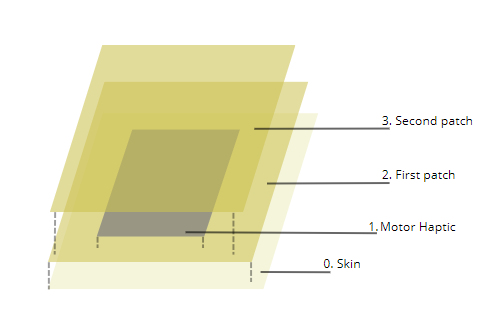
\includegraphics[width=0.5\linewidth]{YOURNAME/images/patch .png}
    \caption{Diagram of the Biopatches and its various layers}
    \label{}
\end{figure}

\section{Evaluation}

\textit{Prostheses}

Regarding prosthetics, a more comprehensive evaluation was conducted. We compared materials and prosthetic manufacturing methods on several aspects:

Multiple printing tests were conducted to determine the easiest-to-use material while providing sufficient quality. In addition to the device for the DIY kit, various types of projects were undertaken, including splints, sockets for amputees, and foot orthoses, to be tested. The standout materials are ABS and PLA. 

Tests of strength and flexibility were performed. Materials offering the most strength in the face of significant mechanical stress are nylon and ABS. However, PP and PETG offer substantial strength due to their flexibility, although PETG can occasionally be too flexible. It is also possible to heat some materials, such as PLA, ABS, and nylon, to reshape the piece and make it more comfortable.

User comfort depends on individual preferences. If the user seeks more mobility, they should opt for a softer prosthesis, while if they prioritize durability, they will choose a sturdier prosthesis.

Considering all these factors, the materials that appear most suitable for the kit's device are ABS and PP. Nevertheless, the choice will depend on the user’s specific needs and intended use. 

\textit{Bio-Patches}

Several tests involving different recipes were conducted. Adjusting the proportions makes it possible to modify the material's elasticity, durability, and resistance to friction. Additionally, obtaining other parameters is conceivable by varying the cooking time and temperature and altering the thickness of the future patch.

Multiple tests were performed, exploring different combinations to achieve the best possible result:

\item Test 1: Place the motor between two layers of gelatin 250, with a smaller layer underneath in contact with the skin and a more significant layer covering the whole. Adherence to the skin is satisfactory, but it may detach in the presence of excessive hair.
\item Test 2: Position the motor between a more extensive upper layer of gelatin 250 and a lower layer of gellan. There is good adherence between the layers but weak adherence to the skin.
\item Test 3: Position the motor between two layers of gelatin 200, with a smaller layer underneath in contact with the skin and a larger layer covering the whole.
\item Test 4: Place the motor between a larger upper layer of gelatin 250 and a lower alginate layer. Alginate adheres well to the skin and serves as an effective lower layer.
\item Test 5: Position the motor between two layers of gelatin 250, with a smaller layer underneath in contact with the skin and a more significant layer covering the whole.
\item Test 6: Place the motor between a more extensive upper layer of gellane and a lower alginate layer.

In summary of the trials conducted with bio-patches, it appears that the larger the lower surface, the stronger the adherence to the skin. Furthermore, if the upper side is smaller than the lower downside, this enhances the cohesion between the two layers and reduces external friction. It is recommended to use gelatin as the material for the lower layer, given its greater flexibility and flexibility compared to other materials, which is particularly crucial for absorbing deformations. To enhance adhesion, it is advisable to moisten both the skin and the patches while ensuring that water droplets are avoided. A significant improvement in adhesion is observed on arms with fewer hairs.

\section{Limitations}
 The prosthetics and design approaches described are preliminary prototypes. They are specifically designed for arm prosthetics and may have limitations depending on the individual's type of amputation. Access to 3D printing and materials can also be a constraint for some individuals.

The biomaterials, patches, and various design methods outlined in this chapter have certain limitations. Despite user-friendliness and affordability, they represent initial attempts and are not designed for long-term durability. They tend to detach and degrade quickly, requiring frequent replacements. Additionally, for optimal effectiveness, it's recommended to have the necessary equipment, including a thermal mixer, which may not be accessible to everyone. Currently, considering the use of commercially available patches is advisable.

\section{Future Works}
It is possible to optimize it by improving the design of the device added to the prosthesis. This approach aims to make it more adaptable to various types of amputations. Furthermore, improvements can be made by exploring multiple materials, seeking to reconcile comfort, flexibility, and strength, and even integrating new innovative materials.

Regarding bio-patches, it is intriguing to explore the development of new bio-patches with a stronger focus on medical models, even though this requires more advanced knowledge and skills, along with higher costs. Additionally, contemplating using new materials such as kombucha presents an opportunity for improvement.

\section{Conclusion}
This chapter represents the first step towards creating a DIY kit to enhance prosthetics. It provides essential knowledge in the fields of prosthetics and biopatches. Through 3D modeling and printing, it becomes possible to integrate the various haptic components discussed in the previous chapter into existing prosthetics. Several concepts and prototypes are presented. Furthermore, this chapter explores the creation of affordable and replicable biopatches accessible to everyone, along with information on testing and results. It also offers insights into manufacturing techniques and material selection for prosthetics and biopatches. 